\section{Incrementally building FAIR Digital Objects with Specimen Data
Refinery
workflows}
\label{ch7:incrementally-building-fair-digital-objects-with-specimen-data-refinery-workflows}

\emph{Specimen Data Refinery} (SDR) is a developing platform for
automating transcription of specimens from natural history collections
\cite{Hardisty 2022} (section \vref{ch8:the-specimen-data-refinery}). SDR is
based on computational workflows and digital twins using FAIR Digital
Objects.

We show our recent experiences with building SDR using the Galaxy
workflow system and combining two FDO methodologies with open digital
specimens (openDS) and RO-Crate data packaging. We suggest FDO
improvements for incremental building of digital objects in
computational workflows.

\subsection{SDR workflows}\label{ch7:sdr-workflows}

\footurl{https://sdr.nhm.ac.uk/}{SDR} is realised as the workflow system
Galaxy \cite{Afgan 2018} with
\footurl{https://github.com/DiSSCo/SDR}{SDR tools} installed. An Open
Research challenge is that some tools have machine learning models with
a commercial licence. This complicates publishing to
\footurl{https://toolshed.g2.bx.psu.edu/}{Galaxy toolshed}, however we
created \footurl{https://www.ansible.com/}{Ansible} scripts to install
equivalent Galaxy servers, including tools and dependencies, accounts
and workflows. SDR workflows are
\footurl{https://workflowhub.eu/projects/72}{published in WorkflowHub} as
FDOs.

We implemented the use case \emph{De novo digitization} in Galaxy \cite{Brack 2022}.
Shown in Figure \vref{ch7:figure1} the
workflow steps exchange openDS JSON \cite{Hardisty 2019}, for
incremental completion of a digital specimen. Initial stages build a
template openDS from a CSV with metadata and image references --
subsequent analysis completes the rest of the JSON with \emph{regions}
of interest, \emph{text} digitised from handwriting, and recognized
\emph{named entities}.

\begin{figure}%[t]
    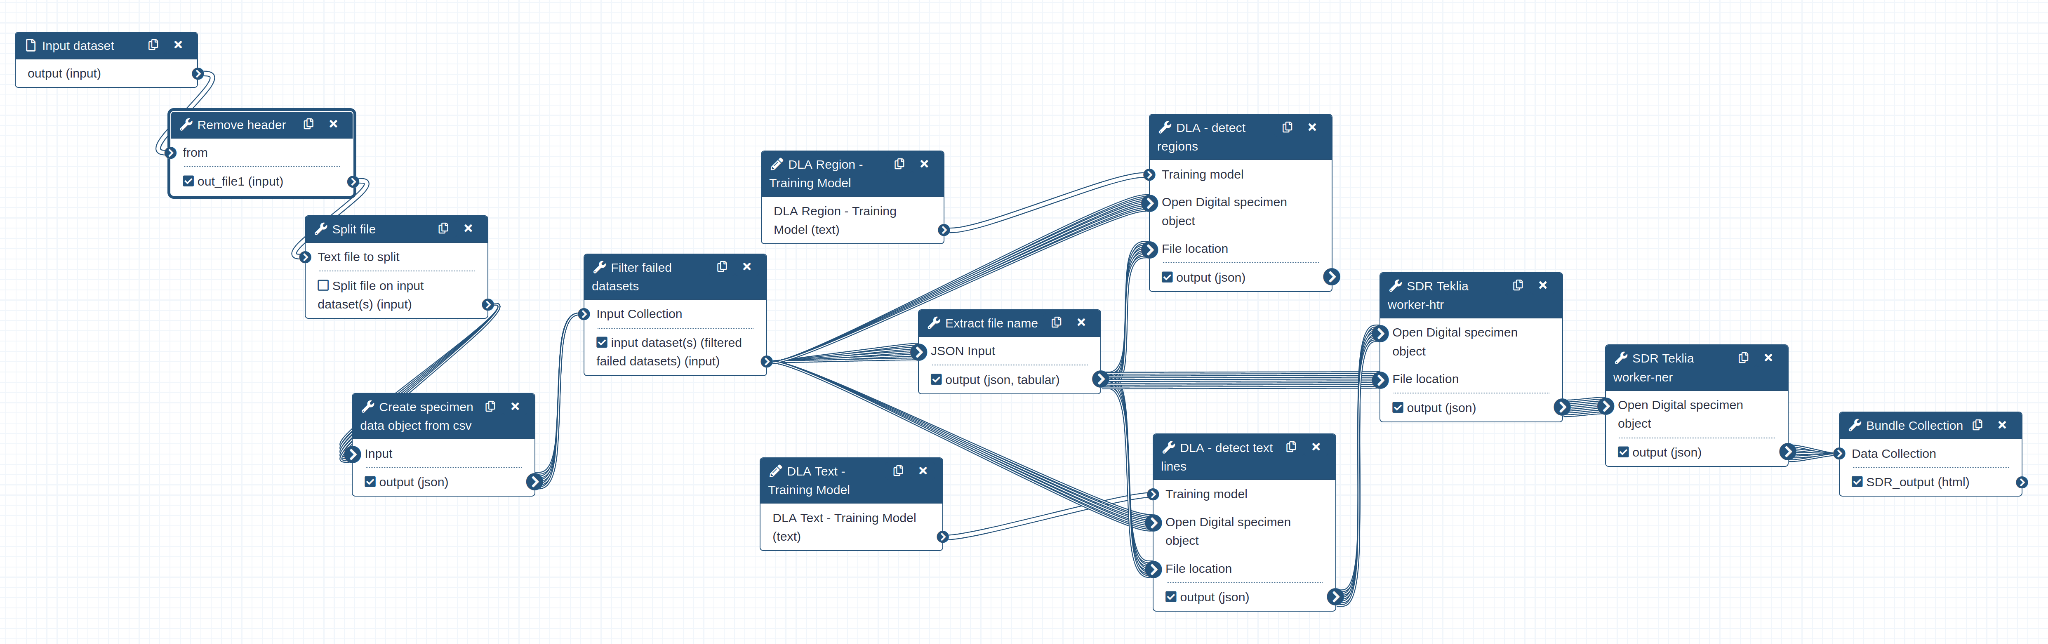
\includegraphics[width=\textwidth]{figures/ch07/figure1.png}
	\caption[FDO propagation in workflow]{\textbf{FDO propagation in workflow}. 
    Draft Galaxy workflow \cite{Brack 2022} 
    shows propagation of partial Open Digital Specimen FDOs between
    individual canonical workflow building blocks. First steps process a CSV
    file to create the initial openDS, where referenced images are analysed
    to detect text lines which are OCRed and then recognized as named
    entities. Bands indicate flow of collections of openDS, processed
    concurrently by each step. The final step bundles the collection of
    openDS FDOs as JSON files in a ZIP archive.}
    \label{ch7:figure1}
  \end{figure}

Galaxy can visualise outputs of each step
(Figure \vref{ch7:figure2}), important to make the
FDOs understandable by domain experts and to verify accuracy of SDR.

\begin{figure}%[t]
    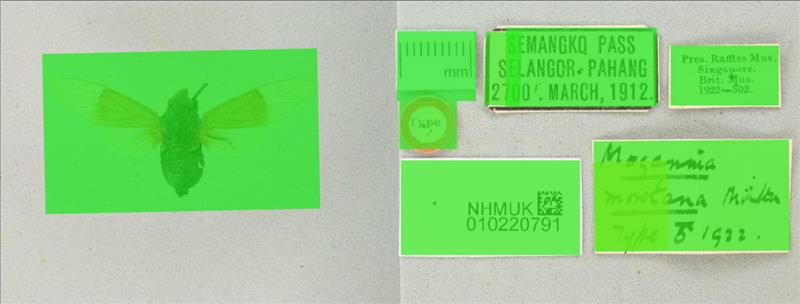
\includegraphics[width=\textwidth]{figures/ch07/figure2.jpg}
	\caption[Visualising openDS FDO within Galaxy]{\textbf{Visualising openDS FDO within Galaxy}.
    Showing detected regions of interest
    (specimen, labels and scale bar) for a pinned insect.}
    \label{ch7:figure2}
\end{figure}

We are adding workflows for partial stages, e.g.~detection of regions
\cite{Livermore 2022a} and hand-written text recognition
\cite{Livermore 2022b}, which we'll combine with scalability testing and wider
testing by project users. Additional workflows will enhance existing
FDOs and use new tools such as barcode detection of museums' internal
identifiers.

We are now ready to publish digital specimens as FAIR Digital Objects,
with registration into \footurl{https://www.dissco.eu/dissco/technical-infrastructure/}{DiSSCO repositories}, PID assignment and workflow provenance. However, even at
this early stage we have identified several challenges that need to be
addressed.

\subsection{FDO lessons}\label{ch7:fdo-lessons}

We highlight the \emph{De novo} use case because this workflow is
exchanging \emph{partial} FDOs -- openDS objects which are not fully
completed and not yet assigned persistent identifiers.
\footurl{https://github.com/DiSSCo/openDS}{openDS schemas} are still in
development, therefore SDR uses a
more flexible
\footurl{https://github.com/DiSSCo/SDR/blob/main/galaxy-workflow/config/opends-schema.json}{JSON schema} where only the initial metadata (populated from CSV) are
required. Each step validates the partial FDO before passing it to the
underlying command line tool.

Although workflow steps exchange openDS objects, they cannot be combined
in any order. For instance, \emph{named entity recognition} requires
digitised text in the FDO. We can consider these intermediate steps as
\emph{sub-profiles} of an FDO Type. Unlike hierarchical subclasses,
these FDO profiles are more like
\footurl{https://en.wikipedia.org/wiki/Duck_typing}{ducktyping}. For
instance a \emph{text detection} step may only require the
\texttt{regions} key, but semantically there is no requirement for say
\texttt{OpenDSWithText} to be a subclass of \texttt{OpenDSWithRegion},
as text also can be transcribed manually without regions.

Similarly, we found that some steps can be executed in parallel, but
this requires merging of partial FDOs. This can be achieved by combining
JSON queries and JSON Schemas, but indicates that it may be more
beneficial to have FDO fragments as separate objects. Adding openDS
fragment steps would however complicate workflows.

Several of our tools process the referenced images, currently https URLs
in openDS. We added a caching layer to avoid repeated image downloading,
coupled with local file-paths wiring in the workflow. A similar
challenge occurs if accessing image data using DOIP, which unlike HTTP,
has no caching mechanisms.

\subsection{RO-Crate lessons}\label{ch7:ro-crate-lessons}

Galaxy is developing support for importing and
exporting \footurl{https://www.researchobject.org/workflow-run-crate/}{Workflow
Run Crates}, a profile of RO-Crate \cite{Soiland-Reyes 2022} to
captures execution history of a workflow, including its definition and
intermediate data \cite{De Geest 2022}. SDR is adopting this support to
combine openDS FDOs with workflow provenance, as envisioned by
\cite{Walton 2020}.

Our prototype \emph{de novo} workflow returns results as a ZIP file of
openDS objects. End-users should also get copies of the referenced
images and generated visualisations, along with workflow execution
metadata. We are investigating ways to embed the preliminary Galaxy
workflow history before the final step, so that this result can be an
enriched RO-Crate.

\subsection{Conclusions}\label{ch7:conclusions}

SDR is an example of machine-assisted construction of FDOs, which
highlight the needs for intermediate digital objects that are not yet
FDO compliant. The passing of such ``local FDOs'' is beneficial not just
for efficiency and visual inspection, but also to simplify workflow
composition of canonical workflow building blocks. At the same time we
see that it is insufficient to only pass FDOs as JSON objects, as they
also have references to other data such as images, which should not need
to be re-downloaded.

Further work will investigate the use of RO-Crate as a wrapper of
partial FDOs, but this needs to be coupled with more flexible FDO types
as profiles, in order to restrict ``impossible'' ordering of steps
depending on particular inner FDO fragments. A distinction needs to be
made between open digital specimens that are in ``draft'' state and
those that can be pushed to DiSSCo registries.

We are experimenting with changing the SDR components into Canonical
Workflow Building Blocks \cite{Soiland-Reyes 2022a}
(\vref{ch6:making-canonical-workflow-building-blocks-interoperable-across-workflow-languages}) 
using the Common Workflow Language \cite{Crusoe 2022}. This gives
flexibility to scalably execute SDR workflows on different compute
backends such as HPC or local cluster, without the additional setup of
Galaxy servers.

